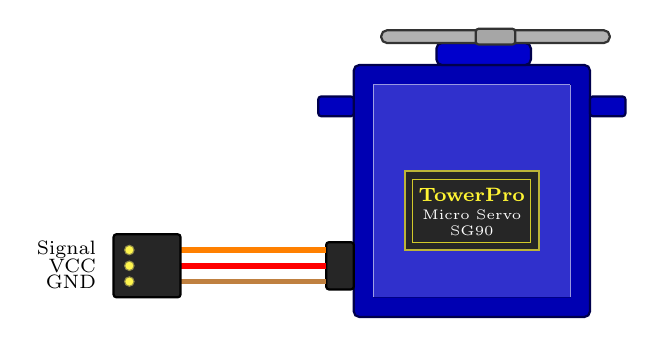
\begin{tikzpicture}[scale=1]
	
	% Hauptgehäuse
	\draw[fill=blue!70!black, draw=blue!30!black, thick, rounded corners=2pt]
	(0,0) rectangle (3.0,3.2);
	
	% Leichte transparente Innenfläche
	\draw[fill=blue!45, draw=blue!20!black, opacity=0.35]
	(0.25,0.25) rectangle (2.75,2.95);
	
	% Schmale Befestigungslaschen oben seitlich
	\draw[fill=blue!75!black, draw=blue!30!black, thick, rounded corners=1pt]
	(-0.45,2.55) rectangle (0,2.80);
	
	\draw[fill=blue!75!black, draw=blue!30!black, thick, rounded corners=1pt]
	(3.0,2.55) rectangle (3.45,2.80);
	
	% Oberes Getriebegehäuse, kleiner
	\draw[fill=blue!80!black, draw=blue!30!black, thick, rounded corners=2pt]
	(1.05,3.2) rectangle (2.25,3.48);
	
	% Servoarm als seitlich betrachteter Rotorarm, länger und ohne Löcher
	\draw[fill=gray!60, draw=gray!40!black, thick, rounded corners=2pt]
	(0.35,3.48) rectangle (3.25,3.64);
	
	% Kleine zentrale Verdickung des Arms
	\draw[fill=gray!70, draw=gray!40!black, thick, rounded corners=1pt]
	(1.55,3.46) rectangle (2.05,3.66);
	
	% Frontlabel
	\draw[fill=black!85, draw=yellow!70!black, line width=0.7pt]
	(0.65,0.85) rectangle (2.35,1.85);
	
	\draw[draw=yellow!80!black, line width=0.4pt]
	(0.75,0.95) rectangle (2.25,1.75);
	
	\node[text=yellow!80!white, font=\scriptsize\bfseries] at (1.5,1.55) {TowerPro};
	\node[text=white, font=\tiny] at (1.5,1.30) {Micro Servo};
	\node[text=white, font=\tiny] at (1.5,1.10) {SG90};
	
	% Gehäusekanten / transparente Details
	\draw[blue!20!white, line width=0.5pt, opacity=0.75]
	(0.25,0.25) -- (0.25,2.95);
	
	\draw[blue!20!white, line width=0.5pt, opacity=0.75]
	(2.75,0.25) -- (2.75,2.95);
	
	\draw[blue!20!white, line width=0.5pt, opacity=0.75]
	(0.25,2.95) -- (2.75,2.95);
	
	% Kabelausgang links unten
	\draw[fill=black!85, draw=black, thick, rounded corners=1pt]
	(0,0.35) rectangle (-0.35,0.95);
	
	% Kabel nach links
	\draw[brown, line width=2pt]
	(-0.35,0.45) -- (-2.2,0.45);
	
	\draw[red, line width=2pt]
	(-0.35,0.65) -- (-2.2,0.65);
	
	\draw[orange, line width=2pt]
	(-0.35,0.85) -- (-2.2,0.85);
	
	% Stecker links
	\draw[fill=black!85, draw=black, thick, rounded corners=1pt]
	(-3.05,0.25) rectangle (-2.2,1.05);
	
	% Kontakte am Stecker
	\draw[fill=yellow!70!white, draw=yellow!50!black]
	(-2.85,0.45) circle (0.06);
	
	\draw[fill=yellow!70!white, draw=yellow!50!black]
	(-2.85,0.65) circle (0.06);
	
	\draw[fill=yellow!70!white, draw=yellow!50!black]
	(-2.85,0.85) circle (0.06);
	
	% Kabelbeschriftung links neben dem Stecker
	\node[font=\scriptsize, anchor=east] at (-3.15,0.45) {GND};
	\node[font=\scriptsize, anchor=east] at (-3.15,0.65) {VCC};
	\node[font=\scriptsize, anchor=east] at (-3.15,0.85) {Signal};
	
\end{tikzpicture}